%\documentclass[handout]{beamer}
\documentclass{beamer}
\usepackage{amsmath}
\usepackage{stdpresent}
%\usepackage[margin=1in]{geometry}
\usepackage{tikz}
\usepackage{natbib}
\usepackage{booktabs}
\usepackage{verbatim}
\usepackage{tikz}
\usetikzlibrary{intersections,positioning}
\usetikzlibrary{matrix, calc}
\newcommand*{\hnode}[1]{\node[outer sep=0pt,anchor=base] (#1) {#1};} 
\usepackage[absolute,overlay]{textpos}
\usetikzlibrary{bayesnet}
\usepackage{tcolorbox}
\usepackage{subfigure}
\usepackage{stackengine}
\usepackage{vimacros}

%\usepackage{subcaption}
\usepackage[tikz]{bclogo}


\newcommand{\cblue}[1]{\textcolor{blue}{{#1}}}
\newcommand{\cred}[1]{\textcolor{red}{{#1}}}

\title[DGM4NLP]{Deep Generative Language Models}
\subtitle{DGM4NLP}

\def\W#1#2{\rnode{#1}{#2}\hfill}

\newcommand{\pointthis}[2]{
        \tikz[remember picture,baseline]{\node[anchor=base,inner sep=0,outer sep=0]%
        (#1) {\textbf{#1}};\node[overlay,rectangle callout,%
        callout relative pointer={(0.1cm,0.5cm)},fill=yellow!90] at ($(#1.north)+(-.5cm,-1cm)$) {#2};}%
        }%

\newcommand{\ack}[1]{\let\thefootnote\relax\footnote{\textcolor{gray}{#1}}}

\presetkeys{bclogo}{
ombre=true,
epBord=3,
couleur = blue!15!white,
couleurBord = red,
arrondi = 0.2,
logo=\bctrombone
}{}

\author[Rios]{Miguel Rios\\University of Amsterdam}
\date{\today}

% add page num
\expandafter\def\expandafter\insertshorttitle\expandafter{%
  \insertshorttitle\hfill%
  \insertframenumber\,/\,\inserttotalframenumber}

\begin{document}
\maketitlepage


\section{Language Modelling}

\frame{ \frametitle{Recap Generative Models of Word Representation}
\begin{textblock*}{\textwidth}(0.1\textwidth,0.25\textheight)
\center Discriminative embedding models\\ \textbf{word2vec} 
\end{textblock*}

\begin{textblock*}{\textwidth}(0.1\textwidth,0.4\textheight)
	\begin{small}
	\begin{center}
	%\only<1>{
	%\emph{\textcolor{blue}{In the event of a chemical spill,} \textcolor{blue}{most children know they should} {\bf evacuate} \textcolor{blue}{as advised by people in} \textcolor{blue}{charge.}}}
	%\only<2-4>{
	\emph{\textcolor{red}{In the event of a chemical spill,} \textcolor{blue}{most children know they should} {\bf evacuate} \textcolor{blue}{as advised by people in} \textcolor{red}{charge.}}
	%}
	%\only<5->{
	%\emph{\textcolor{red}{In the event of a chemical spill,} \textcolor{blue}{most children know they should} \pointthis{evacuate}{ambiguity} \textcolor{blue}{as advised by people in} \textcolor{red}{charge.}}}
	\end{center}
	\end{small}
	\end{textblock*}
	
	
	\begin{textblock*}{\textwidth}(0.2\textwidth,0.6\textheight)
	
	\only<1->{
	Place words in $\mathbb R^d$ as to answer questions like

	\begin{center}	
	\emph{``Have I seen this word in this context?''}
	\end{center}
	}
	
	\only<2->{
	Fit a binary classifier
	\begin{itemize}
		\item \textcolor{blue}{positive} examples
		\item \alert{negative} examples\\ 		
	\end{itemize}
	}
	\end{textblock*}

}

\frame{ \frametitle{Recap Generative Models of Word Representation}
\begin{itemize}

\item The models processes a sentence and outputs a word representation:
\begin{figure}
	\includegraphics[scale=0.40]{elmo-bert-gpt}
\end{figure}


\end{itemize}

}





\frame{ \frametitle{Recap Generative Models of Word Representation}


	\begin{textblock*}{\textwidth}(0.21\textwidth,0.23\textheight)
	\begin{center}
		\textcolor{blue}{quickly evacuate the area} ~ / ~  \textcolor{orange!90!yellow}{deje el lugar r\'{a}pidamente}
	\end{center}
	\end{textblock*}
	
	\begin{textblock*}{0.3\textwidth}(0.025\textwidth,0.35\textheight)
	\scalebox{0.7}{
	%\begin{figure}
%\center
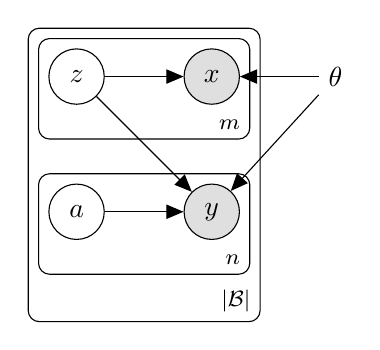
\begin{tikzpicture}
\node[obs]	                   (x)		{$ x $};
\node[obs, below = of x]	       (y)		{$ y $};
\node[latent, left = of x]		(z)		{$ z $};
\node[latent, left = of y]		(a)		{$ a $};
\node[right = of x] (theta) {$\theta$};

% Connect nodes
\edge{a}{y};
\edge{z}{x};
\edge{z}{y};
\edge{theta}{y,x};

% add plates
\plate {L1-sentence} {(x)(z)} {$ m $};
\plate {L2-sentence} {(y)(a)} {$ n $};
\plate {corpus} {(L1-sentence) (L2-sentence)} {$|\mathcal B|$};

\end{tikzpicture}
%\caption{\label{fig:GM2}This model is a refinement of that in \rfig{GM1}, where the latent variable $z$ that participates in generating the aligned sentences. This allows for representations to be ``disambiguated'' in context.}
%\end{figure}
	}
	\end{textblock*}
	
	\begin{textblock*}{\textwidth}(0.32\textwidth,0.35\textheight)
	\begin{figure}
    \begin{overprint}
    \onslide<1>\includegraphics[scale=0.2]{animation/embed1}
    \onslide<2>\includegraphics[scale=0.2]{animation/embed2}
    \onslide<3>\includegraphics[scale=0.2]{animation/embed3}
    \onslide<4>\includegraphics[scale=0.2]{animation/embed4}
    \onslide<5>\includegraphics[scale=0.2]{animation/embed5}
    \onslide<6>\includegraphics[scale=0.2]{animation/embed6}
    \onslide<7>\includegraphics[scale=0.2]{animation/embed7}
    \onslide<8>\includegraphics[scale=0.2]{animation/embed8}
    \onslide<9->\includegraphics[scale=0.2]{animation/embed9} 
    \end{overprint}
\end{figure}
	%\includegraphics[scale=0.2]{animation/embed1}
	%\includegraphics[scale=0.2]{animation/embed2} \pause
	%\includegraphics[scale=0.2]{animation/embed3} \pause
	%\includegraphics[scale=0.2]{animation/embed4} \pause
	%\includegraphics[scale=0.2]{animation/embed5} \pause
	%\includegraphics[scale=0.2]{animation/embed6} \pause
	%\includegraphics[scale=0.2]{animation/embed7} \pause
	%\includegraphics[scale=0.2]{animation/embed8} \pause
	%\includegraphics[scale=0.2]{animation/embed9} \pause
	
	%\begin{small}
	%		\begin{tabular}{p{0.5cm} | p{1.5cm} p{1.5cm} p{1.5cm} p{1.5cm}}
	%		\only<3->{$X$ & \textcolor{blue}{quickly$_1$} & \textcolor{blue}{evacuate$_2$} & \textcolor{blue}{the$_3$} & \textcolor{blue}{area$_4$}} \\
	%		\only<3->{& $\uparrow$ & $\uparrow$ & $\uparrow$ & $\uparrow$} \\
	%		\only<2->{$Z$ & $z_{\textcolor{blue}{1}}$ & $z_{\textcolor{blue}{2}}$ & $z_{\textcolor{blue}{3}}$ & $z_{\textcolor{blue}{4}}$} \\
	%		& & & & \\
	%		\only<4->{$A$ & $a_{\textcolor{orange!90!yellow}{1}}=\textcolor{blue}{2}$ & $a_{\textcolor{orange!90!yellow}{2}}=\textcolor{blue}{3}$ & $a_{\textcolor{orange!90!yellow}{3}}=\textcolor{blue}{4}$ & $a_{\textcolor{orange!90!yellow}{4}}=\textcolor{blue}{1}$ }\\
	%		\only<5->{$Z_a$ & $z_{\textcolor{blue}{2}}$ & $z_{\textcolor{blue}{3}}$ & $z_{\textcolor{blue}{4}}$ & $z_{\textcolor{blue}{1}}$} \\
	%		 \only<6->{& $\downarrow$ & $\downarrow$ & $\downarrow$ & $\downarrow$ } \\
	%		\only<6->{$Y$ & \textcolor{orange!90!yellow}{deje$_1$} & \textcolor{orange!90!yellow}{el$_2$} & \textcolor{orange!90!yellow}{lugar$_3$} & \textcolor{orange!90!yellow}{r\'{a}pidamente$_4$}} \\
		%	\end{tabular}
	%\end{small}
	\end{textblock*}
	
	%\begin{textblock*}{\textwidth}(0.1\textwidth,0.9\textheight)
	%Marginalising alignments collects additional training data for $z$
	%\end{textblock*}


}

\frame[<+->]{ \frametitle{Recap Generative Models of Word Representation}
%\begin{textblock*}{0.35\textwidth}(0.8\textwidth,0.05\textheight)

\begin{figure}
  \includegraphics[width=0.42\textwidth]{architecture.pdf}
 %  \hfill
%   \includegraphics[width=0.42\textwidth]{dec.png}
\end{figure}


%\end{textblock*}

%\begin{textblock*}{\textwidth}(0.05\textwidth,0.15\textheight)
%\begin{itemize}
%\item Embedding 128d
%\item BiLSTM 128d
%\item Z 100d
%\end{itemize}
%\end{textblock*}
}



\frame{ \frametitle{Introduction}
\begin{itemize}
\item 
\end{itemize}

}



\frame[<+->]{ \frametitle{}
\begin{itemize}
\item 

\end{itemize}
}

\frame[<+->]{ \frametitle{}
\begin{itemize}
\item 
\end{itemize}
}

\frame[<+->]{ \frametitle{}
\begin{itemize}
\item 
\end{itemize}
}

\frame[<+->]{ \frametitle{}
\footnotesize{
\begin{itemize}
\item 
\end{itemize}
}
}

\frame[<+->]{ \frametitle{}

\begin{itemize}
\item 
\end{itemize}

}


\frame[<+->]{ \frametitle{}

\begin{itemize}

\item 
\end{itemize}

}




\section{Variational Auto-encoder for Sentences}


\frame[<+->]{ \frametitle{VAE Recap}

\begin{itemize}

\item 

\end{itemize}

}


\frame[<+->]{ \frametitle{}

\begin{itemize}

\item 

\end{itemize}

}

\frame[<+->]{ \frametitle{}

}

%\frame[<+->]{ \frametitle{}
%\begin{itemize}
 
% \item 
%\end{itemize}
%}







\subsection{Model}
%TODO
%\subsection{Motivation}
%\frame[<+->]{ \frametitle{Motivation}
%\begin{block}{Intuition}
%TODO !!!!!
%\end{block}
%}

%\subsection{Model 1}

\frame[<+->]{ \frametitle{}

}








\section*{References}
	
	%
\frame[plain]{
	\frametitle{Earley intersection}
	
	\begin{footnotesize}
	\begin{align*}
	\textsc{Axioms} & \\
	& \drule{}{\itembrack{S' \ra \bullet S, q, q}}{q \in I} \\
	\textsc{Goal} & \\
	& \itembrack{S' \ra S \bullet, q, r} ~ q \in I \wedge r \in F\\
	\textsc{Scan} & \\
	& \drule{\itembrack{X \ra \alpha \bullet x \beta, q, s}}{\itembrack{X \ra \alpha x \bullet \beta}}{\angbrack{s, x, r} \in E}\\
	\textsc{Predict} & \\
	& \drule{\itembrack{X \ra \alpha \bullet Y \beta, q, r}}{\itembrack{Y \ra \bullet \gamma, r, r}}{Y \ra \gamma \in R} \\
	\textsc{Complete} & \\
	& \drule{\itembrack{X \ra \alpha \bullet Y \beta, q, s}\itembrack{Y \ra \gamma \bullet, s, r}}{\itembrack{X \ra \alpha Y_{s,r} \bullet \beta, q, r}}{X \neq S'} \\
	\textsc{Accept} & \\
	& \drule{\itembrack{S' \ra \bullet S, q, q}\itembrack{S \ra \gamma \bullet, q, r}}{\itembrack{S' \ra  S_{q,r} \bullet, q, r}}{r \in F} 
	\end{align*}
	\end{footnotesize}

	
}




	\frame[allowframebreaks]{ \frametitle{References}
	
        \bibliographystyle{plainnat}
        \bibliography{BIB}
	}


\end{document}
\grid
